\documentclass{article}

\usepackage{amsmath, amssymb}
\usepackage{tikz}
\usepackage{graphicx}
\usepackage[margin=1in, landscape]{geometry}
\usetikzlibrary{shapes, arrows, positioning, calc}

\begin{document}

% ---------- Forward ----------
\noindent
\resizebox{\linewidth}{!}{%
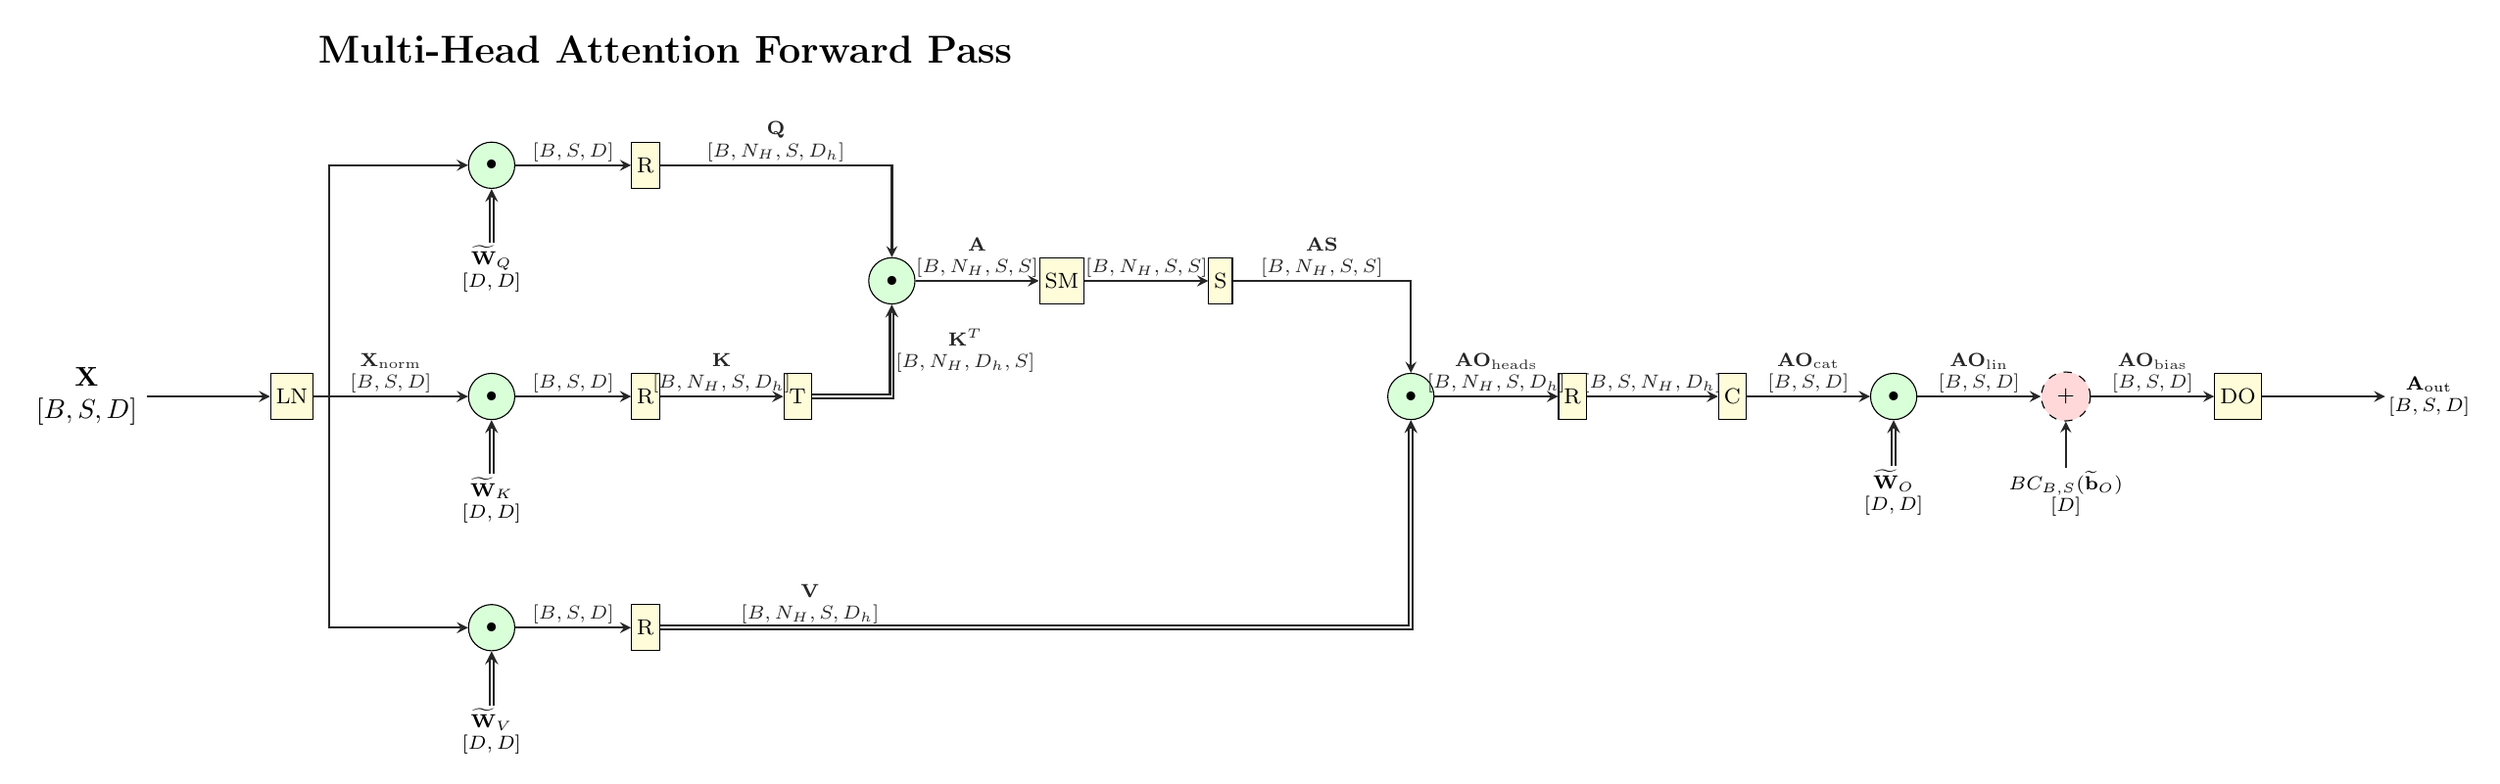
\begin{tikzpicture}[
  every node/.style={transform shape}, % 텍스트도 노드 크기 변화 반영
  >=stealth,
  auxnode/.style={draw, rectangle, fill=yellow!15, minimum height=6mm, inner sep=2pt, font=\footnotesize, align=center},
  mulnode/.style={draw, circle, fill=green!15, minimum size=6mm, font=\footnotesize, align=center},
  addnode/.style={draw, circle, dashed, fill=red!15, minimum size=6mm, font=\footnotesize, align=center},
  flow/.style={->, thick, black!85},
  flow2/.style={->, double, thick, black!85},
  dimlabel/.style={font=\scriptsize, inner sep=1pt, align=center},
  gradflow/.style={->, thick, black!85},
  gradweight/.style={->, thick, black!85}
]
\node[font=\Large\bfseries] at (8, 4.5) {Multi-Head Attention Forward Pass};

\node (Input) at (0.5, 0) [align=center] {$\mathbf{X}$\\$[B,S,D]$};
\node[auxnode] (LN) [right=1.6cm of Input] {LN};

\node[mulnode] (Proj_Q) [right=2.0cm of LN, yshift=3.0cm] {$\bullet$};
\node[auxnode] (R_Q) [right=1.5cm of Proj_Q] {R};

\node[mulnode] (Proj_K) [right=2.0cm of LN, yshift=0cm] {$\bullet$};
\node[auxnode] (R_K) [right=1.5cm of Proj_K] {R};

\node[mulnode] (Proj_V) [right=2.0cm of LN, yshift=-3.0cm] {$\bullet$};
\node[auxnode] (R_V) [right=1.5cm of Proj_V] {R};

\node[dimlabel] (WQ) [align=center, below=0.7cm of Proj_Q] {$\widetilde{\mathbf{W}}_{Q}$\\$[D,D]$};
\node[dimlabel] (WK) [align=center, below=0.7cm of Proj_K] {$\widetilde{\mathbf{W}}_{K}$\\$[D,D]$};
\node[dimlabel] (WV) [align=center, below=0.7cm of Proj_V] {$\widetilde{\mathbf{W}}_{V}$\\$[D,D]$};

\node[auxnode] (T_K) [right=1.6cm of R_K] {T};
\node[mulnode] (QK) [right=2.7cm of R_Q, yshift=-1.5cm] {$\bullet$};
\node[auxnode] (SM) [right=1.6cm of QK] {SM};
\node[auxnode] (Soft) [right=1.6cm of SM] {S};
\node[mulnode] (PV) [right=2.0cm of Soft, yshift=-1.5cm] {$\bullet$};

\node[auxnode] (R_Merge) [right=1.6cm of PV] {R};
\node[auxnode] (Cat) [right=1.7cm of R_Merge] {C};

\node[mulnode] (OProj) [right=1.6cm of Cat] {$\bullet$};
\node[dimlabel] (WO_FWD) [align=center, below=0.6cm of OProj] {$\widetilde{\mathbf{W}}_{O}$\\$[D,D]$};
\node[addnode] (AddB) [right=1.6cm of OProj] {+};
\node[dimlabel] (BO) [align=center, below=0.6cm of AddB] {$BC_{B,S}(\widetilde{\mathbf{b}}_{O})$\\$[D]$};
\node[auxnode] (Drop) [right=1.6cm of AddB] {DO};
\node[dimlabel] (Aout) [align=center, right=1.6cm of Drop] {$\mathbf{A}_{\text{out}}$\\$[B,S,D]$};

\draw[flow] (Input) -- (LN);

\draw[flow] (LN.east) -- ++(0.2,0) |- (Proj_Q.west);
\draw[flow] (LN) -- (Proj_K.west) node[dimlabel, midway, above]{$\mathbf{X}_{\text{norm}}$\\$[B,S,D]$};
\draw[flow] (LN.east) -- ++(0.2,0) |- (Proj_V.west);

\draw[flow2] (WQ) -- (Proj_Q);
\draw[flow2] (WK) -- (Proj_K);
\draw[flow2] (WV) -- (Proj_V);

\draw[flow] (Proj_Q) -- (R_Q) node[dimlabel, midway, above]{$[B,S,D]$};
\draw[flow] (Proj_K) -- (R_K) node[dimlabel, midway, above]{$[B,S,D]$};
\draw[flow] (Proj_V) -- (R_V) node[dimlabel, midway, above]{$[B,S,D]$};

\draw[flow] (R_Q) -| (QK) node[dimlabel, near start, above]{$\mathbf{Q}$\\$[B,N_H,S,D_h]$};
\draw[flow] (R_K) -- (T_K) node[dimlabel, midway, above]{$\mathbf{K}$\\$[B,N_H,S,D_h]$};
\draw[flow2] (T_K) -| (QK) node[dimlabel, near end, right]{$\mathbf{K}^{T}$\\$[B,N_H,D_h,S]$};

\draw[flow] (QK) -- (SM) node[dimlabel, midway, above]{$\mathbf{A}$\\$[B,N_H,S,S]$};
\draw[flow] (SM) -- (Soft) node[dimlabel, midway, above]{$[B,N_H,S,S]$};
\draw[flow] (Soft) -| (PV) node[dimlabel, near start, above]{$\mathbf{AS}$\\$[B,N_H,S,S]$};
\draw[flow2] (R_V) -| (PV) node[dimlabel, pos=0.1, above]{$\mathbf{V}$\\$[B,N_H,S,D_h]$};

\draw[flow] (PV) -- (R_Merge) node[dimlabel, midway, above]{$\mathbf{AO}_{\text{heads}}$\\$[B,N_H,S,D_h]$};
\draw[flow] (R_Merge) -- (Cat) node[dimlabel, midway, above]{$[B,S,N_H,D_h]$};
\draw[flow] (Cat) -- (OProj) node[dimlabel, midway, above]{$\mathbf{AO}_{\text{cat}}$\\$[B,S,D]$};
\draw[flow2] (WO_FWD) -- (OProj);
\draw[flow] (OProj) -- (AddB) node[dimlabel, midway, above]{$\mathbf{AO}_{\text{lin}}$\\$[B,S,D]$};
\draw[flow] (BO) -- (AddB);
\draw[flow] (AddB) -- (Drop) node[dimlabel, midway, above]{$\mathbf{AO}_{\text{bias}}$\\$[B,S,D]$};
\draw[flow] (Drop) -- (Aout);
\end{tikzpicture}%
}

% ---------- Backward ----------
\par\vspace{1cm}
\noindent
\resizebox{\linewidth}{!}{%
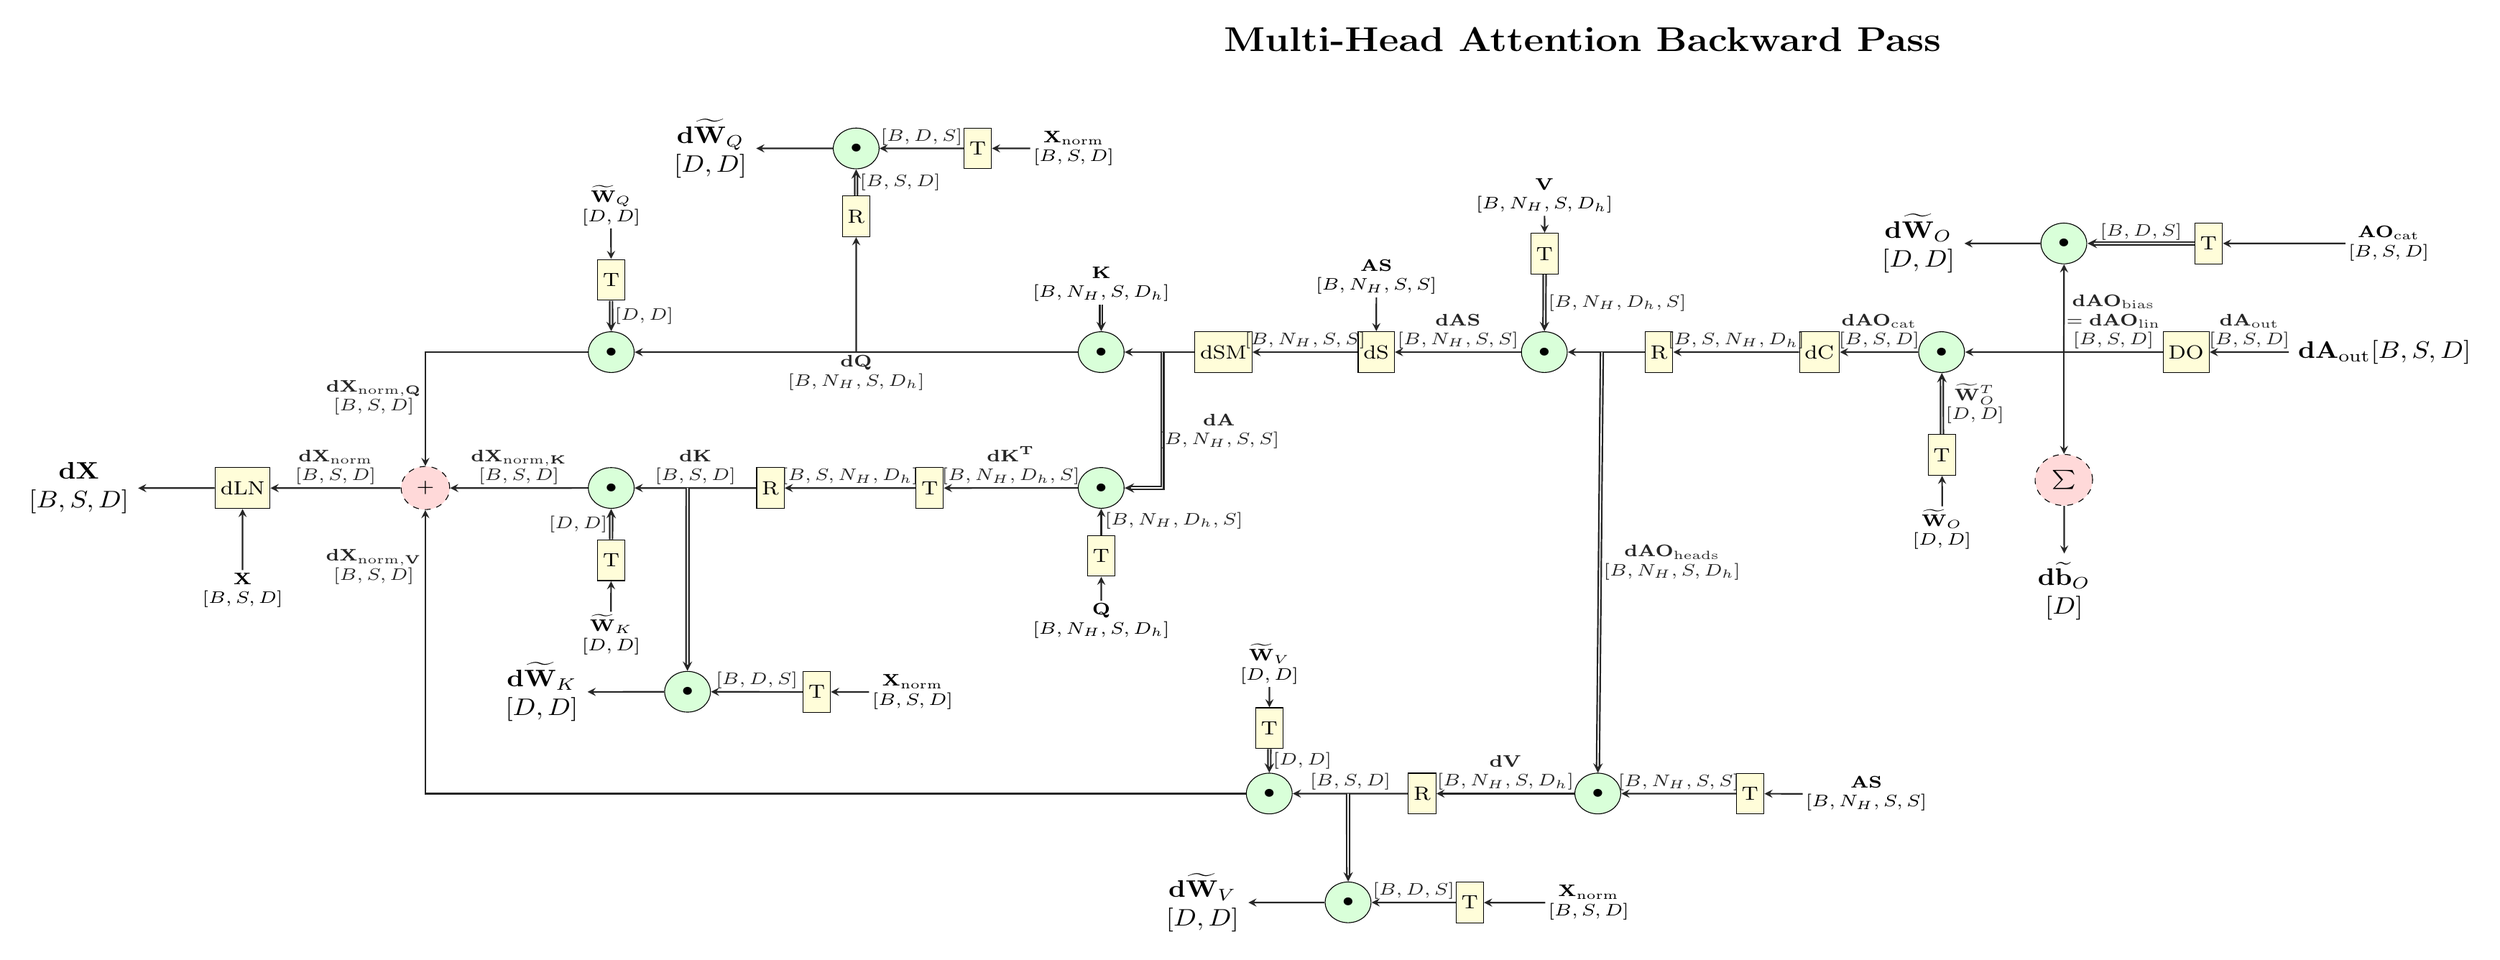
\begin{tikzpicture}[
  every node/.style={transform shape}, % 텍스트도 노드 크기 변화 반영
  >=stealth,
  auxnode/.style={draw, rectangle, fill=yellow!15, minimum height=6mm, inner sep=2pt, font=\footnotesize, align=center},
  mulnode/.style={draw, circle, fill=green!15, minimum size=6mm, font=\footnotesize, align=center},
  addnode/.style={draw, circle, dashed, fill=red!15, minimum size=6mm, font=\footnotesize, align=center},
  flow/.style={->, thick, black!85},
  flow2/.style={->, double, thick, black!85},
  dimlabel/.style={font=\scriptsize, inner sep=1pt, align=center},
  gradflow/.style={->, thick, black!85},
  gradweight/.style={->, thick, black!85}
]

\begin{scope}[xscale=1.35, yscale=1.2]

\def\yoffset{-1.0}
\def\dVXyoffset{-6.5}

\coordinate (Grad_Aout_B) at (17.5, \yoffset);
\coordinate (dDrop_center) at (15.9, \yoffset);
\coordinate (ProjGradSplit) at (14.3, \yoffset);
\coordinate (dOProj_center) at (12.7, \yoffset);
\coordinate (C_center) at (11.1, \yoffset);
\coordinate (R_center) at (9.0, \yoffset);
\coordinate (dPV_AS_calc_center) at (7.5, \yoffset);
\coordinate (dSoft_center) at (5.3, \yoffset);
\coordinate (dSM_calc_center) at (3.3, \yoffset);
\coordinate (dV_calc_center) at (8.2, \dVXyoffset+\yoffset);
\coordinate (R_V_bwd_center) at (5.9, \dVXyoffset+\yoffset);
\coordinate (dVX_calc_center) at (3.9, \dVXyoffset+\yoffset);
\coordinate (dQK_calc_Q_center) at (1.7, \yoffset);
\coordinate (dQK_calc_K_center) at (1.7, -2.0+\yoffset);
\coordinate (K_BWD_input_center) at (1.7, 1.0+\yoffset);
\coordinate (T_Q_bwd_center) at (1.7, -3.0+\yoffset);

\node[font=\Large\bfseries] at (8, 4.6+\yoffset) {Multi-Head Attention Backward Pass};

\node (Grad_Aout_B) at (18.5, \yoffset) {$\mathbf{dA}_{\text{out}}$\\$[B,S,D]$};
\node[auxnode] (DO) at (dDrop_center) {DO};
\node[mulnode] (dOProj) at (dOProj_center) {$\bullet$};

\node[auxnode] (T_WO) [below=0.9cm of dOProj] {T};
\node[dimlabel] (WO_BWD) [below=0.45cm of T_WO] {$\widetilde{\mathbf{W}}_{O}$\\$[D,D]$};

\node[mulnode] (dWO_calc) at ($(ProjGradSplit)+(0, 1.6)$) {$\bullet$};
\node[align=center, left=1.0cm of dWO_calc]
  (dWO_GRAD) {$\mathbf{d}\widetilde{\mathbf{W}}_{O}$\\$[D,D]$};
\node[auxnode] (T_AO_in) [right=1.4cm of dWO_calc] {T};
\node[dimlabel] (AO_in_local_label) [right=1.6cm of T_AO_in] {$\mathbf{AO}_{\text{cat}}$\\$[B,S,D]$};

\node[auxnode] (C) at (C_center) {dC};
\node[auxnode] (R) at (R_center) {R};

\node[mulnode] (dPV_AS_calc) at (dPV_AS_calc_center) {$\bullet$};
\node[auxnode] (dSoft) at (dSoft_center) {dS};
\node[auxnode] (dSM_calc) at (dSM_calc_center) {dSM};

\node[mulnode] (dQK_calc_Q) at (dQK_calc_Q_center) {$\bullet$};
\node[mulnode] (dQX_proj_calc) [left=5.8cm of dQK_calc_Q] {$\bullet$};

\node[mulnode] (dQK_calc_K) at (dQK_calc_K_center) {$\bullet$};
\node[mulnode] (dKX_proj_calc) [left=5.8cm of dQK_calc_K] {$\bullet$};

\node[dimlabel] (K_BWD_input) at (K_BWD_input_center) {$\mathbf{K}$\\$[B,N_H,S,D_h]$};
\node[auxnode] (T_Q_bwd) at (T_Q_bwd_center) {T};
\node[dimlabel] (Q_BWD_input) [below=0.35cm of T_Q_bwd] {$\mathbf{Q}$\\$[B,N_H,S,D_h]$};

\node[dimlabel] (V_FWD) [above=1.7cm of dPV_AS_calc] {$\mathbf{V}$\\$[B,N_H,S,D_h]$};
\node[auxnode] (T_V_bwd) [below=0.25cm of V_FWD] {T};

\node[mulnode] (dV_calc) at (dV_calc_center) {$\bullet$};
\node[auxnode] (T_AS_bwd) [right=1.5cm of dV_calc] {T};
\node[dimlabel] (AS_BWD_for_V) [right=0.5cm of T_AS_bwd] {$\mathbf{AS}$\\$[B,N_H,S,S]$};

\node[auxnode] (R_V_bwd) at (R_V_bwd_center) {R};
\node[mulnode] (dVX_calc) at (dVX_calc_center) {$\bullet$};

\node[auxnode] (T_WV) [above=0.35cm of dVX_calc] {T};
\node[dimlabel] (WV_BWD) [above=0.3cm of T_WV] {$\widetilde{\mathbf{W}}_{V}$\\$[D,D]$};

\node[addnode] (Sum_dBO) [below=1.5cm of ProjGradSplit] {$\sum$};
\node (dBO) [align=center, below=0.7cm of Sum_dBO] {$\mathbf{d}\widetilde{\mathbf{b}}_{O}$\\$[D]$};

\draw[gradflow] (Grad_Aout_B) -- (DO)
  node[dimlabel, midway, above]{$\mathbf{dA}_{\text{out}}$\\$[B,S,D]$};

\draw[gradflow] (DO) -- (dOProj)
  node[dimlabel, pos=0.25, above]{$\mathbf{dAO}_{\text{bias}}$\\$=\mathbf{dAO}_{\text{lin}}$\\$[B,S,D]$};

\draw[gradflow] (ProjGradSplit) -- (dWO_calc.south);
\draw[gradflow] (ProjGradSplit) -- ([yshift=-0.75cm]ProjGradSplit) -| (Sum_dBO.north);

\draw[gradflow] (dOProj) -- (C)
  node[dimlabel, midway, above]{$\mathbf{dAO}_{\text{cat}}$\\$[B,S,D]$};
\draw[gradflow] (C) -- (R)
  node[dimlabel, midway, above]{$[B,S,N_H,D_h]$};

\coordinate (R_split_point) at ($(dPV_AS_calc)!0.5!(R)$);
\draw[gradflow] (R.west) -- (dPV_AS_calc.east);
\draw[flow2] (R_split_point) -- (dV_calc.north)
  node[dimlabel, midway, right]{$\mathbf{dAO}_{\text{heads}}$\\$[B,N_H,S,D_h]$};

\draw[gradflow] (V_FWD.south) -- (T_V_bwd.north);
\draw[flow2] (T_V_bwd.south) -- (dPV_AS_calc.north)
  node[dimlabel, midway, right]{$[B,N_H,D_h,S]$};
\draw[gradflow] (dPV_AS_calc.west) -- (dSoft.east)
  node[dimlabel, midway, above]{$\mathbf{dAS}$\\$[B,N_H,S,S]$};

\node (AS_BWD_dS) [dimlabel, above=0.5cm of dSoft] {$\mathbf{AS}$\\$[B,N_H,S,S]$};
\draw[gradflow] (AS_BWD_dS.south) -- (dSoft.north);
\draw[gradflow] (dSoft.west) -- (dSM_calc.east)
  node[dimlabel, midway, above]{$[B,N_H,S,S]$};

\coordinate (dA_Split_X) at ($(dSM_calc_center)!0.5!(dQK_calc_Q_center)$);
\coordinate (dA_Split) at (dA_Split_X |- dQK_calc_Q.east);
\draw[gradflow] (dSM_calc.west) -- (dQK_calc_Q.east);
\draw[flow2] (dA_Split) -- (dA_Split |- dQK_calc_K.east) -- (dQK_calc_K.east)
  node[dimlabel, pos=-1.5, above, yshift=15]{$\mathbf{dA}$\\$[B,N_H,S,S]$};

\draw[flow2] (K_BWD_input.south) -- (dQK_calc_Q.north);
\draw[gradweight] (dQK_calc_Q) -- (dQX_proj_calc)
  node[dimlabel, midway, below]{$\mathbf{dQ}$\\$[B,N_H,S,D_h]$};

\node[auxnode] (T_WQ_bwd) [above=0.45cm of dQX_proj_calc] {T};
\node[dimlabel] (WQ_bwd) [above=0.45cm of T_WQ_bwd] {$\widetilde{\mathbf{W}}_{Q}$\\$[D,D]$};
\draw[flow] (WQ_bwd) -- (T_WQ_bwd);
\draw[flow2] (T_WQ_bwd.south) -- (dQX_proj_calc.north)
  node[dimlabel, midway, right]{$[D,D]$};

\draw[flow] (Q_BWD_input.north) -- (T_Q_bwd.south);
\draw[flow] (T_Q_bwd.north) -- (dQK_calc_K.south)
  node[dimlabel, pos=0.55, right]{$[B,N_H,D_h,S]$};

\node[auxnode] (T_dK) at ($(dQK_calc_K)!0.35!(dKX_proj_calc)$) {T};
\node[auxnode] (R_dK_mid) at ($(T_dK)!0.5!(dKX_proj_calc)$) {R};

\draw[gradweight] (dQK_calc_K) -- (T_dK)
  node[dimlabel, midway, above]{$\mathbf{dK^T}$\\$[B,N_H,D_h,S]$};
\draw[gradweight] (T_dK) -- (R_dK_mid)
  node[dimlabel, midway, above]{$[B,S,N_H,D_h]$};
\draw[gradweight] (R_dK_mid) -- (dKX_proj_calc)
  node[dimlabel, midway, above]{$\mathbf{dK}$\\$[B,S,D]$};

\node[auxnode] (T_WK_bwd) [below=0.45cm of dKX_proj_calc] {T};
\node[dimlabel] (WK_bwd) [below=0.45cm of T_WK_bwd] {$\widetilde{\mathbf{W}}_{K}$\\$[D,D]$};
\draw[gradflow] (WK_bwd) -- (T_WK_bwd);
\draw[flow2] (T_WK_bwd.north) -- (dKX_proj_calc.south)
  node[dimlabel, midway, left]{$[D,D]$};

\draw[gradflow] (AS_BWD_for_V.west) -- (T_AS_bwd.east);
\draw[gradflow] (T_AS_bwd.west) -- (dV_calc.east)
  node[dimlabel, midway, above]{$[B,N_H,S,S]$};
\draw[gradflow] (dV_calc.west) -- (R_V_bwd.east)
  node[dimlabel, midway, above]{$\mathbf{dV}$\\$[B,N_H,S,D_h]$};
\draw[gradflow] (R_V_bwd) -- (dVX_calc.east)
  node[dimlabel, midway, above]{$[B,S,D]$};

\draw[gradflow] (WV_BWD) -- (T_WV);
\draw[flow2] (T_WV) -- (dVX_calc.north)
  node[dimlabel, midway, right]{$[D,D]$};

\node[addnode] (Sum_dXnorm) [left=1.8cm of dKX_proj_calc] {$+$};

\draw[gradweight] (dQX_proj_calc.west) -| node[dimlabel, pos=0.7, left]{$\mathbf{dX}_{\text{norm},\mathbf{Q}}$\\$[B,S,D]$} (Sum_dXnorm.north);
\draw[gradweight] (dKX_proj_calc.west) -- node[dimlabel, midway, above]{$\mathbf{dX}_{\text{norm},\mathbf{K}}$\\$[B,S,D]$} (Sum_dXnorm.east);
\draw[gradweight] (dVX_calc.west) -| node[dimlabel, pos=0.9, left]{$\mathbf{dX}_{\text{norm},\mathbf{V}}$\\$[B,S,D]$} (Sum_dXnorm.south);

\coordinate (dV_branch) at ($(R_V_bwd.west)!0.52!(dVX_calc.east)$);
\node[mulnode] (dWV_mul) at ($(dV_branch)+(0,-1.6cm)$) {$\bullet$};
\draw[flow2] (dV_branch) -- (dWV_mul.north);

\node[auxnode] (T_Xnorm) [right=1.1cm of dWV_mul] {T};
\node[dimlabel] (Xnorm_local) [right=0.8cm of T_Xnorm] {$\mathbf{X}_{\text{norm}}$\\$[B,S,D]$};
\draw[gradflow] (Xnorm_local) -- (T_Xnorm);
\draw[gradflow] (T_Xnorm.west) -- (dWV_mul.east)
  node[dimlabel, midway, above]{$[B,D,S]$};
\node (dWV_out) [align=center, left=1.0cm of dWV_mul] {$\mathbf{d}\widetilde{\mathbf{W}}_{V}$\\$[D,D]$};
\draw[gradweight] (dWV_mul.west) -- (dWV_out);

\coordinate (dQ_branch) at ($(dQK_calc_Q.east)!0.50!(dQX_proj_calc.west)$);
\node[mulnode] (dWQ_mul) at ($(dQ_branch)+(0,3.0cm)$) {$\bullet$};
\node[auxnode] (R_dQ_for_WQ) at ($(dWQ_mul)+(0,-1.0cm)$) {R};
\draw[gradflow]  (dQ_branch) -- (R_dQ_for_WQ.south);
\draw[flow2] (R_dQ_for_WQ.north) -- (dWQ_mul.south)
  node[dimlabel, midway, right]{$[B,S,D]$};

\node[auxnode] (T_XnormQ) [right=1.1cm of dWQ_mul] {T};
\node[dimlabel] (Xnorm_localQ) [right=0.5cm of T_XnormQ] {$\mathbf{X}_{\text{norm}}$\\$[B,S,D]$};
\draw[gradflow] (Xnorm_localQ) -- (T_XnormQ);
\draw[gradflow] (T_XnormQ.west) -- (dWQ_mul.east)
  node[dimlabel, midway, above]{$[B,D,S]$};
\node (dWQ_out) [align=center, left=1.0cm of dWQ_mul] {$\mathbf{d}\widetilde{\mathbf{W}}_{Q}$\\$[D,D]$};
\draw[gradweight] (dWQ_mul.west) -- (dWQ_out);

\coordinate (dK_branch) at ($(R_dK_mid)!0.52!(dKX_proj_calc)$);
\node[mulnode] (dWK_mul) at ($(dK_branch)+(0,-3.0cm)$) {$\bullet$};
\draw[flow2]  (dK_branch) -- (dWK_mul.north);

\node[auxnode] (T_XnormK) [right=1.2cm of dWK_mul] {T};
\node[dimlabel, right=0.5cm of T_XnormK] (Xnorm_localK) {$\mathbf{X}_{\text{norm}}$\\$[B,S,D]$};
\draw[gradflow] (Xnorm_localK) -- (T_XnormK);
\draw[gradflow] (T_XnormK.west) -- (dWK_mul.east)
  node[dimlabel, midway, above]{$[B,D,S]$};
\node (dWK_out) [align=center, left=1.0cm of dWK_mul] {$\mathbf{d}\widetilde{\mathbf{W}}_{K}$\\$[D,D]$};
\draw[gradweight] (dWK_mul.west) -- (dWK_out);

\draw[gradweight] (Sum_dBO) -- (dBO);

\draw[gradflow] (WO_BWD) -- (T_WO);
\draw[flow2] (T_WO) -- (dOProj)
  node[dimlabel, midway, right]{$\widetilde{\mathbf{W}}_{O}^{T}$\\$[D,D]$};
\draw[gradflow] (AO_in_local_label) -- (T_AO_in);
\draw[flow2] (T_AO_in) -- (dWO_calc.east)
  node[dimlabel, midway, above]{$[B,D,S]$};
\draw[gradweight] (dWO_calc) -- (dWO_GRAD);

\node[auxnode] (dLN) [left=1.7cm of Sum_dXnorm] {dLN};
\draw[gradweight] (Sum_dXnorm.west) -- node[dimlabel, midway, above]
  {$\mathbf{dX}_{\text{norm}}$\\$[B,S,D]$} (dLN.east);

\node (dX_OUT) [align=center, left=1.0cm of dLN] {$\mathbf{dX}$\\$[B,S,D]$};
\draw[gradweight] (dLN.west) -- (dX_OUT);

\node[dimlabel] (LNCache) [below=0.9cm of dLN] {$\mathbf{X}$\\$[B,S,D]$};
\draw[gradflow] (LNCache.north) -- (dLN.south);

\end{scope}
\end{tikzpicture}
}


% =========================
% Abbreviation Tables for MHA Diagrams (new page)
% =========================
\newpage
\renewcommand{\arraystretch}{1.2}
\small

% -------- Operations (Ops) --------
\begin{center}
\textbf{Operations (Ops)}
\begin{tabular}{llll}
\hline
\textbf{Abbrev} & \textbf{Name} & \textbf{Type / Shape} & \textbf{Notes} \\
\hline
LN  & Layer Normalization           & op & Normalizes per token (per last dim $D$). \\
DO  & Dropout                       & op & Training-time stochastic dropout. \\
$+$ & Bias Add                      & op & Adds broadcast bias; see $\mathrm{BC}_{B,S}(\cdot)$. \\
T   & Transpose                     & op & Context-dependent dims (e.g., $[B,N_H,S,D_h]\!\to\![B,N_H,D_h,S]$). \\
R   & Reshape / Split / Merge       & op & Head split/merge: $[B,S,D]\!\leftrightarrow\![B,N_H,S,D_h]$. \\
C   & Concatenate                   & op & Join heads along last dim: $[B,S,N_H,D_h]\!\to\![B,S,D]$. \\
SM  & Scale (+ Mask)                & op & Multiply by $1/\sqrt{D_h}$ and apply mask to scores. \\
S   & Softmax                       & op & Softmax over key length ($S$) per head. \\
$\mathrm{BC}_{B,S}(\cdot)$ & Broadcast & op & Broadcast a length-$D$ (or $D_h$, $V$) bias to $[B,S,\cdot]$. \\
dS  & Softmax Backward              & op & Backprop through softmax over $S$. \\
dSM & Scale/Mask Backward           & op & Backprop through scaling and masking. \\
dC  & De-concatenate (Backward)     & op & Split grads from concatenated heads. \\
dLN & LayerNorm Backward            & op & Uses cached LN stats ($\mu,\sigma$) and $\mathbf{X}$. \\
\hline
\end{tabular}
\end{center}

\vspace{0.8em}

% -------- Data Tensors (Values) --------
\begin{center}
\textbf{Data Tensors (Values)}
\begin{tabular}{llll}
\hline
\textbf{Symbol} & \textbf{Name} & \textbf{Shape} & \textbf{Notes} \\
\hline
$\mathbf{X}$                 & Input hidden states           & $[B,S,D]$       & Into MHA block (pre-LN). \\
$\mathbf{X}_{\text{norm}}$   & LN output                     & $[B,S,D]$       & Result of LN($\mathbf{X}$). \\
$\mathbf{Q},\mathbf{K},\mathbf{V}$ & Query/Key/Value         & $[B,N_H,S,D_h]$   & From linear projections of $\mathbf{X}_{\text{norm}}$. \\
$\widetilde{\mathbf{W}}_{Q}$ & Q weight                      & $[D,D]$         & Per-head realized by reshape; drawn as single matmul. \\
$\widetilde{\mathbf{W}}_{K}$ & K weight                      & $[D,D]$         & Same convention. \\
$\widetilde{\mathbf{W}}_{V}$ & V weight                      & $[D,D]$         & Same convention. \\
$\widetilde{\mathbf{W}}_{O}$ & Output-proj weight            & $[D,D]$         & Maps concatenated heads back to model dim. \\
$\widetilde{\mathbf{b}}_{O}$ & Output bias                   & $[D]$           & Broadcast via $\mathrm{BC}_{B,S}$. \\
$\mathbf{A}$                 & Attention scores              & $[B,N_H,S,S]$     & $\mathbf{Q}\mathbf{K}^T/\sqrt{D_h}$ (plus mask). \\
$\mathbf{AS}$                & Attention weights             & $[B,N_H,S,S]$     & $\mathrm{softmax}(\mathbf{A})$. \\
$\mathbf{AO}_{\text{heads}}$ & Per-head outputs              & $[B,N_H,S,D_h]$   & $\mathbf{AS}\cdot\mathbf{V}$. \\
$\mathbf{AO}_{\text{cat}}$   & Concatenated heads            & $[B,S,D]$       & After \textit{C}. \\
$\mathbf{AO}_{\text{lin}}$   & Linear output                 & $[B,S,D]$       & $\mathbf{AO}_{\text{cat}}\widetilde{\mathbf{W}}_{O}$. \\
$\mathbf{AO}_{\text{bias}}$  & Bias-added output             & $[B,S,D]$       & $\mathbf{AO}_{\text{lin}}+\widetilde{\mathbf{b}}_{O}$. \\
$\mathbf{A}_{\text{out}}$    & MHA output                    & $[B,S,D]$       & After dropout; to next sublayer. \\
\hline
$\mathbf{dA}_{\text{out}}$   & Grad wrt MHA output           & $[B,S,D]$       & Backprop signal entering MHA. \\
$\mathbf{dQ},\mathbf{dK},\mathbf{dV}$ & Gradients for Q/K/V & $[B,N_H,S,D_h]$   & From attention-core backward. \\
$\mathbf{dK^T}$              & Grad of $K^T$                 & $[B,N_H,D_h,S]$   & Before transpose/reshape to $\mathbf{dK}$. \\
$\mathbf{dAO}_{\text{heads}}$& Grad at heads                 & $[B,N_H,S,D_h]$   & Split from $\mathbf{dAO}_{\text{cat}}$. \\
$\mathbf{dX}_{\text{norm},Q}$& Grad wrt $X_{\text{norm}}$ (Q branch) & $[B,S,D]$ & Contribution via $W_Q^T$. \\
$\mathbf{dX}_{\text{norm},K}$& Grad wrt $X_{\text{norm}}$ (K branch) & $[B,S,D]$ & Contribution via $W_K^T$. \\
$\mathbf{dX}_{\text{norm},V}$& Grad wrt $X_{\text{norm}}$ (V branch) & $[B,S,D]$ & Contribution via $W_V^T$. \\
$\mathbf{dX}_{\text{norm}}$  & Sum of above                  & $[B,S,D]$       & Input to dLN. \\
$\mathbf{dX}$                & Grad wrt input $X$            & $[B,S,D]$       & Output of dLN. \\
$\mathbf{d}\widetilde{\mathbf{W}}_{Q}$ & Q weight grad      & $[D,D]$         & Standard matmul rule. \\
$\mathbf{d}\widetilde{\mathbf{W}}_{K}$ & K weight grad      & $[D,D]$         & Standard matmul rule. \\
$\mathbf{d}\widetilde{\mathbf{W}}_{V}$ & V weight grad      & $[D,D]$         & From reshaped $d\mathbf{V}$ and $X_{\text{norm}}$. \\
$\mathbf{d}\widetilde{\mathbf{W}}_{O}$ & Output-proj grad   & $[D,D]$         & From $\mathbf{AO}_{\text{cat}}^T$ and $d\mathbf{AO}_{\text{lin}}$. \\
$\mathbf{d}\widetilde{\mathbf{b}}_{O}$ & Output bias grad   & $[D]$           & Sum over $B,S$ of $d\mathbf{AO}_{\text{lin}}$. \\
\hline
\multicolumn{4}{l}{\textbf{Shape symbols:}\; $B$=batch size,\; $S$=sequence length,\; $D$=model dim,\; $N_H$=num heads,\; $D_h=D/N_H$.} \\
\multicolumn{4}{l}{\textbf{Implementation note:}\; Per-head $[D,D]$ drawings depict fused linears realized via reshape to $N_H\times D_h$.} \\
\hline
\end{tabular}
\end{center}

\end{document}
